% {{{=================== Introduction ======================


\section{Introduction}

\subsection{Motivation}
\UH{}\footnote{Unknown Horizons website: \url{http://www.unknown-horizons.org}} is an \OS{} real-time strategy game developed by a team of programmers, artists, game
designers and many more around the globe. The first revision to the current project was committed in late 2007\footnote{First commit to \UH{}:
\url{https://github.com/unknown-horizons/unknown-horizons/commit/53eec12fd8bb52ac1a6ccfdb097296c479499dfd}}. The idea
started out in 2005 under the name \textit{OpenAnno} and was renamed to \UH{} in 2008.

Over the years the project grew to a small team of more than 10 active developers and many
patch contributers. The recent release version of \UH{} has been downloaded more than 10000 times\footnote{Sourceforge
download statistics:
\url{http://sourceforge.net/projects/unknownhorizons/files/Unknown\%20Horizons/2011.2/}}\footnote{Chip.de download
statistics: \url{http://www.chip.de/downloads/Unknown-Horizons_33713541.html\#sp=unknown horizons\&N=0\&pos=1}}, a rather
big user-base compared to the team size.

In this document I want to give a personal report on the work I have done on \UH{} in the past years and give an
overview of how certain parts of the project's organization have evolved.

\subsection{About Me}
My name is Thomas Kinnen, I'm currently doing my Masters in Computer Science. On the development team and in the code
repository I am mostly known by the nick-name \textit{nihathrael}.

I started working on the project in early 2008, shortly after the first commits had been commited to the repository. 
The project had come to a nearly complete halt when I joined, so I set out to bring it back to life.

Since November 2008 I am one of the two project coordinators, with focus on code direction and introduction of new
potential members to the team and code. In this position I got a good view into most of the necessary parts of an \OS{}
game development team. This includes public relations, mentoring new members, graphics, content, programming, code
design, leading meetings and many more in the context of an \OS{} game.

\section{History}
In this section I present the history before and during my time as part of the \UH{} team. I will give only a brief
overview of the history before I joined the project as the current state has nothing but the idea in common with the
older versions.

\subsection{Pre History}
The idea for the \UH{} project existed long before I joined the team in 2008. The project's first name was \textit{OpenAnno}
for which the original sourceforge.net project was registered as early as July 2005\footnote{Original sourceforge.net
project: \url{http://sourceforge.net/projects/openanno/}}. The original announcement for OpenAnno can be found on the
german linux forums: \url{http://linuxforen.de/forums/showthread.php?t=188350}. Version 3.5 (See screenshot in \figref{oascreenshot}) of OpenAnno was released in
early 2006\footnote{Link to a download site: \url{http://happypenguin.org/newsitem?id=6154}}. After a rewrite to C++,
version 0.0.1.0 of OpenAnno was released in September 2006\footnote{Release announcement 0.0.1.0:
\url{http://da.zfx.info/developia/viewarticlecomments.php?cid=28999\#29101}}. 

\begin{figure}[!htb]
	\begin{center}
		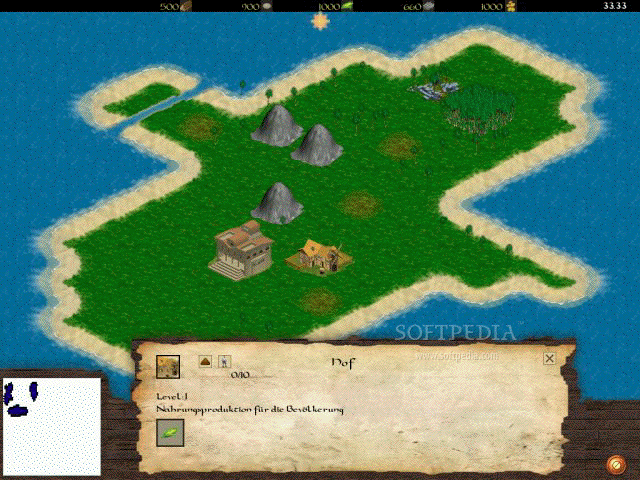
\includegraphics[scale=0.50]{pics/openannoscreenshot}
	\end{center}
    \caption{Early screenshot from OpenAnno 3.5 - taken from
    \href{http://mac.softpedia.com/progScreenshots/OpenAnno-Screenshot-13550.html}{Softpedia.com}}
    \label{oascreenshot}
\end{figure}

In April 2007 \textit{LinuxDonald}(Thomas Kowaliczek) took over the project from
\textit{The Brain}(Martin Gerhardy)\footnote{Original Blogpost by LinuxDonald (German):
\url{http://www.linuxdonald.de/blog/?p=4}}.

The project took an interesting turn in August 2007 when the team decided to
split the project into a 2D and a 3D version\footnote{Splitting 2D/3D blogpost:
\url{http://www.linuxdonald.de/blog/?p=13}}.

OpenAnno 2D was restarted in September 2007, using FIFE\footnote{FIFE
website \url{httpd//www.fifengine.net}} as its graphics engine. The team was hoping the collaboration with a dedicated
graphics engine would make their work easier, as they had previously stalled on implementing different terrain hights
and where having trouble getting all the work done. OpenAnno 3D was dropped in the same decision as the team had
realized that the burden of developing two games basically in parallel was not a viable option. This presented a radical
cut in the development of OpenAnno, as the core repository had over 1000 commits at that time\footnote{Blogpost about
the 1000th commit: \url{http://www.linuxdonald.de/blog/?p=6}}. Restarting meant throwing years of development over board
to start again from scratch.

\subsection{History - 2008}
In March 2008 I joined the project as a novice programmer. When I joined the project had almost come to a halt, amazed
by the idea of writing an \OS{} game in the footsteps of \textit{Anno 1602} I decided to give it a try non-the-less. The
entire code was removed and I started from scratch, using only the graphics we had. Motivated by the new start
\textit{spq} quickly joined me in my efforts only 18 days later. spq and I had a lot of time at our disposal, so with
the help of many other old and new members development of \textit{OpenAnno} progressed quickly, we hit 500 commits to the repository
by June 2008 and finished our first milestone 2008.1 by July 8th. The 1000. commit followed quickly by July 16th. At the
end of July the team had its first meetup at the \textit{Dusmania 2008} hobby game developers conference and was awarded
2nd place in the category best game.

On the October 1st \textit{OpenAnno} hit a major milestone with its first public release: Version 2008.1. The release
received quite a lot of coverage and was featured on some big websites like the german magazine chip.de\footnote{Chip newsentry to
2008.1:\url{http://www.chip.de/news/OpenAnno-Strategiespiel-Klassiker-als-Open-Source_33713075.html\#sp=openanno&N=0&pos=1}}
and the freegamer blog\footnote{Freegamer blogpost: \url{http://freegamer.blogspot.com/2008/10/lavirinto-3d-060-balazar-3-01-openanno.html}}

During this time it became clear that \textit{LinuxDonald} would not be able to continue doing the project management
due to a lack of time on his side. After a long meeting and a vote at the beginning of November it was decided to split the
position in two team coordinator jobs. \textit{Nightraven} (Tobias Schröfel) was assigned to public relations and
advertising and guiding game design decisions. I was chosen to assign tasks and guide the development of the codebase.
Tasks for both project coordinators were defined as posting news updates, guiding discussion on IRC and helping new
interested developers join our project. LinuxDonald agreed to continue hosting the website and repository
infrastructure, showing it was not the lack of interest but the lack time that caused him to step down.

\subsection{History - 2009}
The year 2009 started with a big change: The project was renamed to \UH{}. This was done for two reasons:
\begin{itemize}
    \item Copyright concerns about the word "Anno" being licensed by \textit{Sunflowers} in Germany
    \item Seperate the game from the original Anno series, underlining it not being a clone
\end{itemize}

As \UH{} is not a formal organization or company any lawsuits against the name (or any other port of the project) would
result in the lawsuit going against the project leaders Nightraven and/or me. Therefor we decided to change the name to
something completely new, leaving us on the safe side of things.

This is the original commit from the official repository performing the renaming:
\begin{lstlisting}[caption=Commit 1831 renaming OpenAnno to Unknown Horizons, label=renamecommit]
Author: nihathrael
Date:   Fri Feb 20 16:39:37 2009 +0000
    * Renamed all accurances of OpenAnno to Unknown Horizons
    * openanno.py is now named run_uh.py
    * openanno.sqlite ist now named game.sqlite
    * Goodbye OpenAnno ;( Off to new shores we go :)
\end{lstlisting}

Besides this big change, 2009 was a regular development year for \UH{}. The team released three new versions of \UH{}:
\begin{itemize}
\item \textit{2009.0}
\item \textit{2009.1}
\item \textit{2009.2} + bugfix release \textit{2009.2a}. 
\end{itemize}
The releases generated over 35 thousand downloads on sourceforge alone.

The release 2009.2 was featured in the big german computer magazine \textit{c't}\footnote{\url{http://www.heise.de/software/download/cdd_95_9}} and was delivered with the magazine's
dvd shipped with each copy. 

\subsection{History - 2010}
In 2010 the team decided to move away from the subversion\footnote{\url{http://subversion.tigris.org}} revision control
system and switch to git\footnote{\url{http://git-scm.com/}}. With this switch, the repository hosting was also moved to
\href{http://www.github.com}{github.com}. Github is a collaborative source-code hosting website which deeply integrates
git into the website. It makes it easy for developers to submit patches and even easier for the team to merge it. This
also moves the source-code hosting away from our own servers, making it much more reliable and cheaper.

The team only released one release: Version \textit{2010.1}. It introduced a network mode, allowing the player
to play with other players over the internet or a local area network.

\subsection{History - 2011}
2011 has been an exciting year for \UH{} so far. Early 2011 the team decided to apply for the \textit{Google Summer of
Code}\footnote{Official GSoC website: \url{http://www.google-melange.com/gsoc/homepage/google/gsoc2011}} program. The
application was accepted and \UH{} was granted 3 student slots. The team had applied together with the graphics engine
FIFE and it was decided that 1 slot would go to FIFE and 2 to \UH{}. The three students which were chosen, were chosen
for the following projects:
\begin{itemize}
    \item Artificial Intelligence Player for \UH{}
    \item Combat for \UH{}
    \item Performance Improvements for the Rendering Pipeline in \textit{FIFE}
\end{itemize}
Before the students started their work, the team released version \textit{2011.1} of \UH{}.

The three students did excellent work during the 3 months of their active work on both \UH{} and \textit{FIFE} and all
easily passed the final evaluation. Following up on the \textit{Summer of Code} Google invited two members of each
organization to participate in the mentor summit at their campus in Mountain View. Christoph Ölmüller, who did the
administrative work for GSoC for \UH{}, and me got the chance to go and meet many fellow \OS{} game developers
from other projects like \BOW{}, \textit{Worldforge} and \textit{Hedgewars}.

\textit{FIFE} released version \textit{0.3.3} of their engine on October 7th,
followed by bugfix release \textit{0.3.3r2} on November 2nd. This release includes all changes done by their student
\textit{kozmo} (Kajetan Świerk). \UH{} will release \UH{} version 2011.2 during the 2nd week of November, containing all
changes made during the \textit{Summer of Code} and the regular development.









\subsection{Problem Statement}

\subsection{Project Context}

%}}}

